\documentclass{ximera}

\input{../../preamble.tex}

\author{Kenneth Berglund}

\begin{document}
Consider the polynomial $q(x) = (x - 3)(-x + 2)^2(-2x - 1)$. 

\begin{exercise}
$q$ has $\answer{3}$ roots.

\begin{exercise}
The roots of $q$ in increasing order are $\answer{-\frac{1}{2}}$, $\answer{2}$, and $\answer{3}$.

\begin{exercise}
The multiplicity of $-\frac{1}{2}$  as a root of $q$ is $\answer{1}$.

The multiplicity of 2 as a root of $q$ is $\answer{2}$. 

The multiplicity of 3 as a root of $q$ is $\answer{1}$. 

\begin{exercise}
The degree of $q$ is \wordChoice{\choice{odd}\choice[correct]{even}}.

The leading coeffficient of $q$ is \wordChoice{\choice{positive}\choice[correct]{negative}}.

As $x \to -\infty$, $q(x) \to$ \wordChoice{\choice{$\infty$}\choice[correct]{$-\infty$}}. As $x \to \infty$, $q(x) \to$ \wordChoice{\choice{$\infty$}\choice[correct]{$-\infty$}}.

\begin{exercise}
Choose the graph of $q(x)$ from the options below.

\begin{image}
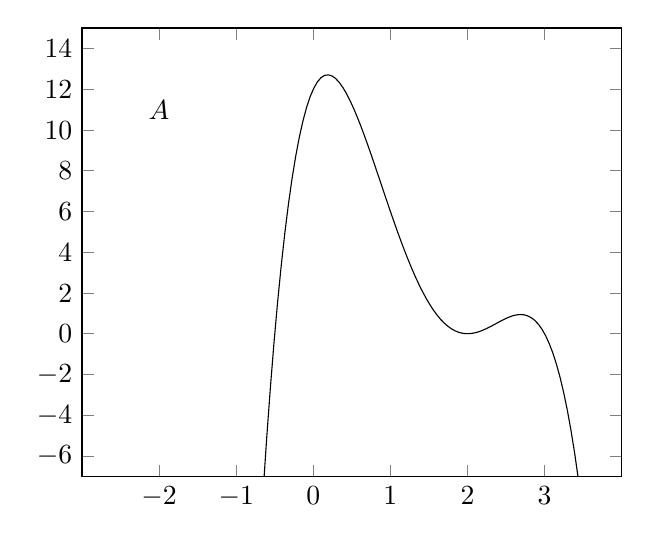
\begin{tikzpicture}
    \begin{axis}[xmin=-3, xmax=4, ymin=-7, ymax=15,
xtick ={-2, -1, ..., 3},
ytick ={-6, -4, ..., 14}]
         \addplot[<->, domain=-3:4,samples=150]{(x - 3)*(-x + 2)^2*(-2*x - 1)} node{};
	\node(label) at (axis cs:-2,11) {$A$};	
    \end{axis}
\end{tikzpicture}
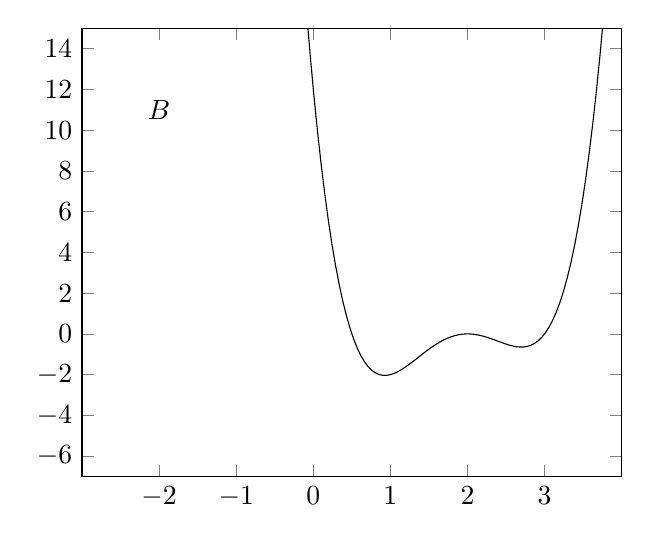
\begin{tikzpicture}
    \begin{axis}[xmin=-3, xmax=4, ymin=-7, ymax=15,
xtick ={-2, -1, ..., 3},
ytick ={-6, -4, ..., 14}]
         \addplot[<->, domain=-3:4,samples=150]{(x - 3)*(-x + 2)^2*(2*x - 1)} node{};
	\node(label) at (axis cs:-2,11) {$B$};	
    \end{axis}
\end{tikzpicture}
\end{image} 

\begin{image}
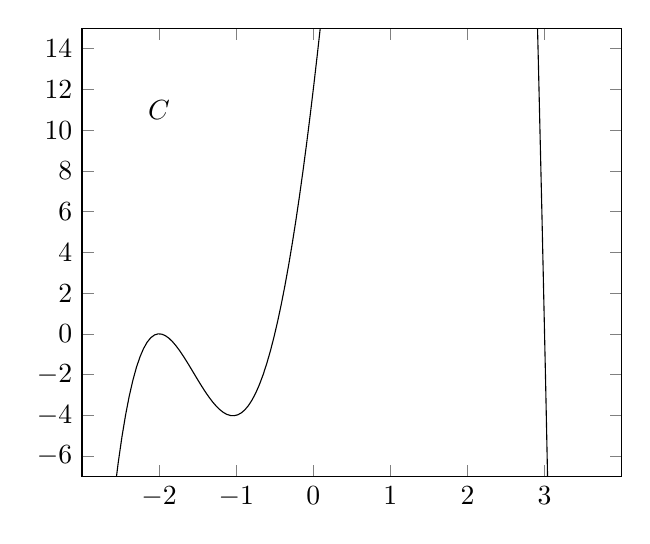
\begin{tikzpicture}
    \begin{axis}[xmin=-3, xmax=4, ymin=-7, ymax=15,
xtick ={-2, -1, ..., 3},
ytick ={-6, -4, ..., 14}]
         \addplot[<->, domain=-3:4,samples=150]{(x - 3)*(x + 2)^2*(-2*x - 1)} node{};
	\node(label) at (axis cs:-2,11) {$C$};	
    \end{axis}
\end{tikzpicture}
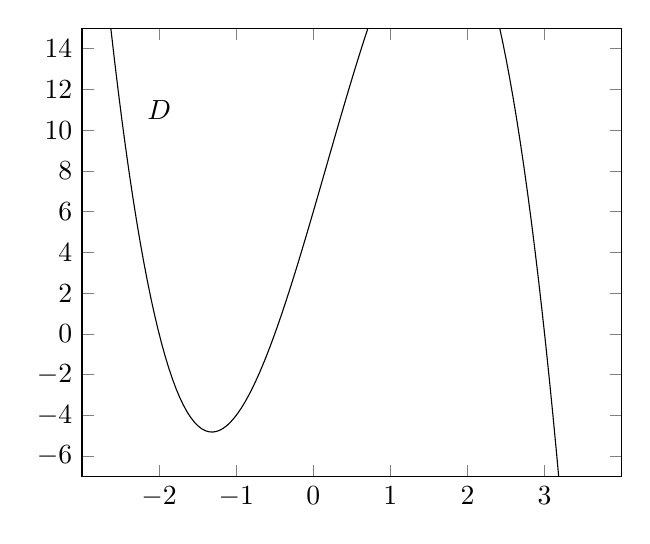
\begin{tikzpicture}
    \begin{axis}[xmin=-3, xmax=4, ymin=-7, ymax=15,
xtick ={-2, -1, ..., 3},
ytick ={-6, -4, ..., 14}]
         \addplot[<->, domain=-3:4,samples=150]{(x - 3)*(x + 2)*(-2*x - 1)} node{};
	\node(label) at (axis cs:-2,11) {$D$};	
    \end{axis}
\end{tikzpicture}
\end{image} 

\begin{multipleChoice}
\choice[correct]{A}
\choice{B}
\choice{C}
\choice{D}
\end{multipleChoice}
\end{exercise}
\end{exercise}
\end{exercise}
\end{exercise}
\end{exercise}


\end{document}